% 0. Preliminares. 
% Esto es voluntario. 
% Consiste en poner lo que ya sabías, porque lo has dado en el grado, y que te haga falta 
% (por ejemplo, algebra lineal, cuerpos finitos, operaciones con polinomios, algoritmos genéticos, etc).

% TODO

\chapter{Preliminares}

En este capítulo se desarrollarán las herramientas necesarias para poder afrontar el criptosistema de McEliece que precisa este trabajo. Empezaremos abordando concepto de anillo y algunas de sus propiedades más importantes. A partir de este noción, podremos definir los cuerpos finitos y los conceptos relacionados con ellos, tales como los anillos de polinomios sobre cuerpos finitos y su utilidad para construir cuerpos finitos. También será de especial relevancia tratar los conceptos relacionados con la teoría de la complejidad para clasificar los problemas de acuerdo a su dificultad. Finalmente, estudiaremos las metaheurísticas basadas en la población para introducir los algoritmos genéticos.

\section{Anillos}

En esta sección introduciremos el concepto de anillo para poder definir el concepto de cuerpo, así como las principales propiedades de esta estructura algebraica.

\begin{definition}
    Un \emph{anillo} $(A, +, \cdot )$ es un conjunto $A$ junto con dos operaciones binarias $A \times A \rightarrow A$ denotadas por la suma (denotada por $+$) y producto (denotado por $\cdot$) que verifican los siguientes axiomas:

    \begin{itemize}
        \item Propiedad asociativa de la suma: 
        $$  a + (b + c) = (a + b) + c \qquad \forall a,b,c \in A$$
        \item Existencia del elemento neutro para la suma:
        $$ 0 + a = a = a + 0 \qquad \forall a \in A$$
        \item Existencia del elemento inverso para la suma:
        $$ \forall a \in A \; \; \exists -a \in A \quad a + (-a) = 0 = (-a) + a $$
        \item Propiedad conmutativa de la suma:
        $$ a + b = b + a \qquad \forall a,b \in A $$
        \item Propiedad asociativa del producto:
        $$ a \cdot (b \cdot c) = (a \cdot b) \cdot c \qquad \forall a,b,c \in A $$
        \item Propiedad distributiva del producto:
        $$ a \cdot (b + c) = a \cdot b + a \cdot c, \quad (b + c) \cdot a = b \cdot a + c \cdot a \qquad \forall a,b,c \in A $$
        
    \end{itemize}

    Un anillo de llama \emph{conmutativo o abeliano} si se verifica la propiedad conmutativa del producto 
    $$ ab = ba \qquad \forall a,b \in A $$
\end{definition}

Es fácil comprobar que en todo anillo se verifica $0 \cdot x = x \cdot 0 = 0$ (obsérvese que $0 \cdot = (0 + 0) \cdot x = 0 \cdot x + 0 \cdot x$ y simplifíquese por el simétrico de $0 \cdot x$).

Además del anillo conmutativo, existen otros casos particulares de anillos. Diremos que un anillo es \emph{unitario} si es un anillo cuyo producto tiene elemento neutro, esto es, $\exists 1 \in A \; : \; x \cdot 1 = 1 \cdot x = x$, para todo $x \in A$.

Diremos que un elemento $a$ del anillo $A$ es \emph{invertible} si existe un elemento $a'$ en el anillo $A$ tal que $a \cdot a' = a' \cdot a = 1$. Este elemento $a'$ es único, lo llamaremos \emph{elemento inverso} y lo denotaremos por $a^{-1}$.

Cuando se da la igualdad $1 = 0$, diremos que el anillo es \emph{trivial} y tendrá un solo elemento.

\begin{definition}
    Sea $A$ un anillo, $1 \in A$ el elemento neutro del producto y $n \geq 1$ un número natural, definimos la cardinalidad de $A$ como:

    \[
        Car(A) = \left\{ \begin{array}{lc}
        0 &   \textit{si } n \cdot 1 \neq 0 \textit{ para cualquier } n \geq 1 \\
        \\ n & \textit{si n es el menor número natural no nulo para el que } n \cdot 1 = 0
        \end{array}
        \right.
    \]
\end{definition}

%TODO
% - Añadir homomorfismo de anillos? (apuntes de álgebra I)
% - Añadir subestructuras de anillos e ideales? (apuntes de álgebra I)
% - Añadir propiedades de los dominios de integridad? (apuntes de álgebra I)

\section{Cuerpos finitos}

Para presentar el concepto de cuerpo finito, necesitaremos definir previamente el concepto de cuerpo junto con algunas de sus propiedades más relevantes.

\begin{definition}
    Un \emph{cuerpo} $(K, +, \cdot)$ es un anillo conmutativo no trivial en el que todo elemento no nulo tiene un inverso multiplicativo. Se dice que un cuerpo es \emph{finito} si tiene un número finito de elementos.
\end{definition}

Sea $(K, +, \cdot)$ un cuerpo y $E \subset K$, diremos que $E$ es un \emph{subcuerpo} de $K$ o $K$ es una \emph{extensión} de $E$ si se cumple que $(E, +, \cdot)$ es un cuerpo cuando las operaciones $+$ y $\cdot$ se restringen a $E$.

Diremos que la \emph{característica} de un cuerpo es el número de elementos que tiene.

Todos los cuerpos finitos tienen un número de elementos $q = p^n$, para algún número primo $p$ y algún entero positivo $n$. Denotaremos por $\mathbb{F}_q$ a los cuerpos finitos con característica $q$, aunque otra común notación es $GF(q)$.

Observemos que si $p$ un número primo y $q$ es un número entero tal que $q = p^n$, entonces $\mathbb{F}_q$ es un espacio vectorial sobre $\mathbb{F}_p$ de dimensión $n$. Además, hay $q$ vectores en el espacio vectorial de dimensión $n$ sobre $\mathbb{F}_p$.

Notemos que todos los cuerpos finitos de orden $q$ son isomorfos, aunque cada cuerpo puede tener diferentes representaciones.

\begin{proposition}
    Sea $\mathbb{F}_q$ un cuerpo finito con $q = p^n$ elementos, entonces 

    $$p \cdot \alpha = 0, \qquad \forall \alpha \in \mathbb{F}_q.$$
\end{proposition}

\begin{proposition}
    Sea $\mathbb{F}_q$ un cuerpo finito con característica $p$, se cumple que

    $$( \alpha + \beta )^p = \alpha^p + \beta^p, \qquad \forall \alpha, \beta \in \mathbb{F}_q.$$
\end{proposition}

% TODO: homomorfismo de cuerpos

\subsection{Anillo de polinomios sobre cuerpos finitos}

En esta sección vamos a introducir el concepto de polinomio junto con sus operaciones.

\begin{definition}
    Sea $A$ un anillo conmutativo. El \emph{conjunto de polinomios} en la variable $x$ con coeficientes en $A$ está compuesto por el siguiente conjunto
    $$\{ a_n x^n  + a_{n-1} x^{n-1} + \cdots + a_1 x + a_0 \; : \; a_0, ..., a_n \in A \}.$$
    Este conjunto se representa por $A[X]$.
\end{definition}

En el conjunto de polinomios definimos una suma y un producto. 

Sean $f = a_n x^n + a_{n-1} x^{n-1} + \cdots + a_1 x + a_0$ y $g = b_m x^m + b_{m-1} x^{m-1} + \cdots + b_1 x + b_0$ dos polinomios. Supongamos que $m \leq n$, tomando $b_i = 0$ para todo $n \geq i > m$, definimos las operaciones de suma y producto de polinomios:

$$f + g = (a_n + b_n)x^n + (a_{n-1} + b_{n-1})x^{n-1} + \cdots + (a_1 + b_1)x + (a_0 + b_0).$$
$$f \cdot g = a_n b_m x^{n+m} + (a_n b_{m+1} + a_{n-1} b_m) x^{n+m-1} + \cdots + (a_1 b_0 + a_0 b_1)x + a_0 b_0.$$

De esta forma, diremos que el conjunto $A[X]$ con las operaciones anteriores es un \emph{anillo de polinomios en X con coeficientes en A}.

\begin{definition}
    Para un polinomio $f = a_n + a_{n-1} x^{n-1} + \cdots + a_1 x + a_0 \neq 0$ el mayor índice $n$ tal que $a_n \neq 0$ se llama \emph{grado de f} y se representa por $\gr(f)$. Si $f = 0$ definimos $\gr(f) = - \infty$.

    Llamaremos \emph{término (de grado i)} a cada uno de los sumandos $a_i X^i$ del polinomio $f$. El \emph{término líder} es el término no nulo de mayor grado. El coeficiente $a_n \neq 0$ del término líder se llama \emph{coeficiente líder} y el término de grado cero $a_0$ se llama \emph{término constante}. Si el coeficiente líder es $1$, diremos que el polinomio es \emph{mónico}.
\end{definition}

A continuación tenemos algunas propiedades de los polinomios.

\begin{proposition}
    Sea $A$ un anillo conmutativo y sean $f,g \in A[X]$ dos polinomios, tenemos que 
    $$\gr(f + g) \leq \max{(\gr(f), \; \gr(g))},$$
    $$\gr(f \cdot g) \leq \gr(f) + \gr(g)$$
    Si $\gr(f) \neq \gr(g)$, se verifica 
    $$\gr(f + g) = \max{(\gr(f), \; \gr(g))}$$
\end{proposition}

Podemos trasladar estos resultados al caso de los cuerpos finitos. Sea $\mathbb{F}_q$ un cuerpo finito, un polinomio $f(x)$ estará definido sobre dicho cuerpo si es de la forma $f(x) = \sum_{i = 0}^{n} a_i \cdot x^i$, donde $a_i \in \mathbb{F}_q$ para todo $i = 0, ..., n$. Análogamente, diremos que $f(x) \in \mathbb{F}_q$.

Sean $f(x)$ y $g(x)$ polinomios en $\mathbb{F}_q[x]$, diremos que $f(x)$ divide a $g(x)$ si existe un polinomio $h(x) \in \mathbb{F}_q[x]$ tal que $g(x) = f(x) h(x)$ y lo denotaremos por $f(x) \vert g(x)$. El polinomio $f(x)$ se llama \emph{divisor} o \emph{factor} de $g(x)$.

El \emph{mayor común divisor} de $f(x)$ y $g(x)$ es el polinomio mónico en $\mathbb{F}_q[x]$ con mayor grado que divide a $f(x)$ y a $g(x)$. Este polinomio es único y se denota por $\mcd(f(x), \; g(x))$. Diremos que los polinomios $f(x)$ y $g(x)$ son \emph{primos relativos} si $\mcd(f(x), \; g(x)) = 1$.

El siguiente resultado es de gran utilidad, pues sirve para calcular los divisores de un polinomio e incluso para calcular el máximo común divisor. Nos dará las bases para definir posteriormente el Algoritmo de Euclides.

\begin{theorem}
    \label{th:div_alg}
    Sean $f(x)$ y $g(x)$ polinomios en $\mathbb{F}_q[x]$ con $g(x)$ no nulo.
    \begin{itemize}
        \item Existen dos polinomios únicos $c(x), r(x) \in \mathbb{F}_q[x]$ tales que
        $$f(x) = g(x) c(x) + r(x), \qquad \textit{donde } \gr(r(x)) < \gr(g(x)) \textit{ o } r(x) = 0.$$
        \item Si $f(x) = g(x) c(x) + r(x)$, entonces $\mcd(f(x), \; g(x)) = \mcd(g(x), \; r(x))$.
    \end{itemize}
\end{theorem}

Los polinomios $c(x)$ y $r(x)$ se llaman \emph{cociente} y \emph{resto}, respectivamente.

Usando este resultado de forma recursiva, obtendremos el máximo común divisor de los polinomios $f(x)$ y $g(x)$. Este procedimiento se conoce como \emph{Algoritmo de Euclides}. El siguiente resultado describe este algoritmo.

\begin{theorem}[Algoritmo de Euclides]
    Sean $f(x)$ y $g(x)$ polinomios definidos en $\mathbb{F}_q[x]$ con $g(x)$ no nulo.
    \begin{enumerate}
        \item Realizar los siguientes pasos hasta que $r_n(x) = 0$ para algún $n$:
        $$f(x) = g(x) c_1(x) + r_1(x), \qquad \textit{donde } \gr(r_1(x)) < \gr(x),$$
        $$g(x) = r_1(x) c_2(x) + r_2(x), \qquad \textit{donde } \gr(r_2(x)) < \gr(r_1),$$
        $$r_1(x) = r_2(x) c_3(x) + r_3(x), \qquad \textit{donde } \gr(r_3(x)) < \gr(r_2),$$
        $$\vdots$$
        $$r_{n-3}(x) = r_{n-2}(x) c_{n-1}(x) + r_{n-1}(x), \qquad \textit{donde } \gr(r_{n-1}(x)) < \gr(r_{n-2}),$$
        $$r_{n-2}(x) = r_{n-1}(x) c_{n}(x) + r_{n}(x), \qquad \textit{donde } r_n(x) = 0.$$
        Entonces $\mcd(f(x), \; g(x)) = cr_{n-1}(x)$, donde $c \in \mathbb{F}_q$ es una constante para que $c r_{n-1}(x)$ sea mónico.
        \item Existen polinomios $a(x), b(x) \in \mathbb{F}_q[x]$ tales que 
        $$a(x) f(x) + b(x) g(x) = \mcd(f(x), \; g(x)).$$
    \end{enumerate}
\end{theorem}

En cada paso el grado del resto se decrementa al menos en $1$, por lo que podemos asegurar que la secuencia de pasos anterior terminará en algún momento.

A continuación se muestran algunos resultados relevantes.

\begin{proposition}
    Sean $f(x)$ y $g(x)$ polinomios en $\mathbb{F}_q[x]$.
    \begin{itemize}
        \item Si $k(x)$ es un divisor de $f(x)$ y $g(x)$, entonces $k(x)$ es un divisor de $a(x) f(x) + b(x) g(x)$ para algunos $a(x), b(x) \in \mathbb{F}_q[x]$.
        \item Si $k(x)$ es un divisor de $f(x)$ y $g(x)$, entonces $k(x)$ es un divisor de $\mcd(f(x), \; g(x))$.
    \end{itemize}
\end{proposition}

\begin{proposition}
    Sea $f(x)$ un polinomio en $\mathbb{F}_q[x]$ de grado $n$.
    \begin{itemize}
        \item Si $\alpha \in \mathbb{F}_q$ es una raíz de $f(x)$, entonces $x - \alpha$ es un factor de $f(x)$.
        \item El polinomio $f(x)$ tiene como mucho $n$ raíces en cualquier cuerpo que contenga a $\mathbb{F}_q$.
    \end{itemize}
\end{proposition}

\begin{theorem}
    Los elementos de $\mathbb{F}_q$ son las raíces de $x^q - x$.
\end{theorem}

\subsubsection{Construcción de cuerpos finitos}

Para realizar la construcción de cuerpos finitos, previamente necesitaremos conocer el siguiente concepto y algunos resultados relacionados.

\begin{definition}
    Sea $f(x) \in \mathbb{F}_q[x]$ un polinomio no constante, decimos que es \emph{irreducible} sobre $\mathbb{F}_q$ si no se factoriza como producto de dos polinomios en $\mathbb{F}_q[x]$ de menor grado.
\end{definition}

\begin{theorem}
    Sea $f(x)$ un polinomio no constante. Entonces

    $$f(x) = p_1(x)^{a_1} \cdots p_k(x)^{a_k},$$

    donde cada $p_i(x)$ es irreducible y único salvo orden, y los elementos $a_i$ son únicos.
\end{theorem}

Como consecuencia de este resultado, tenemos que $\mathbb{F}_q[x]$ es un \emph{dominio de factorización única}.

El siguiente resultado nos muestra cómo construir un cuerpo finito de característica $p$ a partir del cociente de anillos de polinomios por polinomios irreducibles.

\begin{proposition}
    Sea $p$ un número primo y sea el polinomio $f(x) \in \mathbb{F}_p[x]$ irreducible en $\mathbb{F}_p$ y de grado $m$. Tenemos que el anillo cociente $\mathbb{F}_q[x]/\left(f(x)\right)$ es un cuerpo finito con $q = p^m$ elementos, es decir, con característica $p$.
\end{proposition}

Escribiremos los elementos del anillo cociente, que son las clases laterales $g(x) + (f(x))$ como vectores en $\mathbb{F}_p^m$ con la siguiente correspondencia:

\begin{equation}
    \label{pr:correspondencia}
    g_{m-1} x^{m-1} + g_{m-2} x^{m-2} + \cdots + g_{1} x + g_0 + (f(x)) \leftrightarrow (g_{m-1}, g_{m-2}, ..., g_1, g_0).
\end{equation}

Esta notación facilita la operación de sumar dos elementos. Sin embargo, la multiplicación es algo más complicada. Supongamos que queremos multiplicar $g_1(x) + (f(x))$ por $g_2(x) + (f(x))$. Para ello, usaremos el resultado \ref{th:div_alg} para obtener

\begin{equation}
    \label{pr:multiplicacion_clase_lateral}
    g_1(x) g_2(x) = f(x) h(x) + r(x),
\end{equation}

donde $\gr(r(x)) \leq m - 1$ o $r(x) = 0$. Entonces 

$$(g_1(x) + (f(x))) (g_2(x) + (f(x))) = r(x) + (f(x)).$$

Podemos simplificar la notación si reemplazamos $x$ por $\alpha$ donde $f(\alpha) = 0$. Por \ref{pr:multiplicacion_clase_lateral}, se cumple que $g_1(\alpha) g_2(\alpha) = r(\alpha)$ y la correspondencia \ref{pr:correspondencia} queda como sigue

$$g_{m-1} g_{m-2} \cdots g_1 g_0 \leftrightarrow  g_{m-1} \alpha^{m-1} g_{m-2} \alpha^{m-2}\cdots g_1 \alpha g_0.$$

De esta forma, multiplicamos los polinomios en $\alpha$ de forma usual y aplicamos al resultado que $f(\alpha) = 0$ para reducir las potencias de $\alpha$ mayores que $m-1$ a polinomios en $\alpha$ de grado menor que $m$.


\section{Teoría de la complejidad}

El objetivo de esta sección se basa en clasificar los problemas de acuerdo a su dificultad. Nos centraremos en estudiar la complejidad de los problemas decidibles, es decir, los problemas que pueden tener algoritmos para resolverlos.

\subsection{Complejidad de los algoritmos}

A la hora de resolver un problema con un algoritmo, tendrán gran importancia los recursos que consume dicho algoritmo, sobre todo el espacio y el tiempo. La complejidad del tiempo de un algoritmo es el número de pasos que necesita para resolver un problema de tamaño $n$. La complejidad de un algoritmo siempre se define en el peor de los casos, esto es, se obtiene una cota para el recuento de los pasos en el peor de los casos. 

La siguiente definición nos proporciona la notación más importante en el análisis de los algoritmos.

\begin{definition}[Notación $\mathcal{O}$-grande]
    Sean $f, g : \mathbb{N}^r \longrightarrow \mathbb{R}$. Decimos que $f(n) = O(g(n))$ si existen dos constantes $c \in \mathbb{R}^+$ y $n_0 \in \mathbb{N}^r$ tales que $\forall n \geq n_0$, $f(n) \leq c \cdot g(n)$.
\end{definition}

Con esta notación podemos analizar el tiempo esperado que va a tardar un algoritmo en realizar una tarea.

\begin{proposition}
    Para cualquier $\lambda \in \mathbb{R}^+$ y $g : \mathbb{N}^r \longrightarrow \mathbb{R}$, tenemos que

    $$\mathcal{O}(g(n)) = \mathcal{O}(\lambda g(n)), \qquad \forall n \in \mathbb{N}^r.$$
\end{proposition}

A continuación presentaremos algunos conceptos importantes para especificar la complejidad de los algoritmos que nos serán de utilidad más adelante.

\begin{definition}[Algoritmo en tiempo polinomial]
    Un algoritmo es un \emph{algoritmo en tiempo polinomial} si su complejidad es $\mathcal{O}(p(n))$, donde $p(n)$ es una función polinómica de $n$.
\end{definition}

\begin{definition}[Algoritmo en tiempo exponencial]
    Un algoritmo es un \emph{algoritmo en tiempo exponencial} si su complejidad es $\mathcal{O}(c^n)$, donde $c$ es una constante real estrictamente mayor que $1$.
\end{definition}

\subsection{Complejidad de los problemas}

La complejidad de un problema es equivalente a la complejidad del mejor algoritmo que resuelve ese problema. Diremos que un problema es \emph{fácil} si existe un algoritmo en tiempo polinomial que lo resuelve, mientras que un problema será \emph{difícil} si no existe ningún algoritmo en tiempo polinomial que lo resuelva.

La teoría de la complejidad de los problemas se ocupa de los \emph{problemas de decisión}. Un problema de decisión siempre tiene una respuesta de sí o no.

\begin{figure}[H]   
	\center
	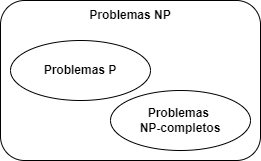
\includegraphics[scale=0.5]{figures/Complejidad.png}
	\caption{Clases de complejidad de los problemas de decisión.}
    \label{fg:complexity}
\end{figure}

Con la teoría computacional podemos clasificar los problemas en sus clases de complejidad. Existen dos clases importantes de problemas: P y NP (Figura \ref{fg:complexity}).

La clase de complejidad P representa a la familia de problemas de decisión que se pueden resolver mediante un algoritmo en tiempo polinomial. Los problemas que pertenecen a esta clase son \emph{fáciles} de resolver.

La clase de compejidad NP representa a la familia de problemas de decisión que se pueden resolver por un algoritmo no determinista en tiempo polinomial. Un algoritmo no determinista tiene algunos puntos en los que hay múltiples combinaciones diferentes sin ninguna especificación de cuál se tomará. Estos problemas se dicen que son más \emph{difíciles} de resolver.

Para definir la clase de los problemas NP-completos, necesitaremos previamente definir el concepto de reducción.

\begin{definition}[Reducción polinómica]
    Un problema de decisión $A$ se \emph{reduce polinómicamente} a otro problema de decisión $B$ si, para todas las instancias de entrada $I_A$ de $A$, siempre se puede construir una instancia de entrada $I_B$ para $B$ en una función de tiempo polinomial, de tal forma que $I_A$ es una instancia positiva de $A$ si y solo si $I_B$ es una instancia positiva de $B$.
\end{definition}

Un problema de decisión es \emph{NP-completo} si es NP y cualquier otro problema de NP se reduce a él. Los problemas que pertenecen a esta clase son los \emph{más difíciles} dentro de la clase NP.

La figura \ref{fg:complexity} muestra la relación entre los problemas P, NP y NP-completos.

Los problemas \emph{NP-duros} son problemas de optimización cuyo problema de decisión asociado es NP-completo. Las metaheurísticas constituyen una importante alternativa para resolver esta clase de problemas.

\section{Metaheurísticas basadas en la población}

Las \emph{metaheurísticas} representan una familia de técnicas de optimización aproximada. Proporcionan soluciones aceptables en un tiempo razonable para resolver problemas difíciles y complejos, esto es, problemas que no pertenecen a la clase de complejidad P o que no se conoce que pertenezcan a dicha clase. Sin embargo, no garantizan la optimalidad de las soluciones obtenidas.

Las \emph{metaheurísticas basadas en la población} se pueden ver como una mejora iterativa en una población de soluciones. Estas metaheurísticas consisten en inicializar la población, posteriormente generan una nueva población de soluciones y finalmente esta nueva población reemplaza a la actual usando algunos procedimientos de selección. Una vez se alcanza la condición dada, el proceso de búsqueda finaliza y obtenemos una solución.

El esquema de este procedimiento se muestra a continuación.

\begin{Ualgorithm}[H]
    \small
    \DontPrintSemicolon
    \KwOut{Mejor solución encontrada}
    $P \longleftarrow P_0$ \tcp{Generación de la población inicial}
    $t \longleftarrow 0$\;
    \While{No se cumpla la condición de parada}{
        Generar($P_t'$) \tcp{Generación de la nueva población}
        $P_{t+1} \longleftarrow $ SeleccionarPoblación($P_t \cup P_t'$) \tcp{Selección de la nueva población}
        $t \longleftarrow t + 1$\;
    }
\end{Ualgorithm}

Vamos a estudiar en detalle este procedimiento concretando los conceptos en los que se basa.

\begin{enumerate}
    \item \textbf{Generación de la población inicial}. Las metaheurísticas basadas en la población comienzan con una población inicial de soluciones. Este paso juega un papel fundamental en la efectividad del algoritmo y su eficiencia. El principal criterio para generar la población es que haya diversidad.
    \item \textbf{Generación de una nueva población}. En este paso, se genera una nueva población de soluciones. Se puede realizar de varias formas, sin embargo la que estudiaremos será la que se basa en la evolución. En esta categoría, las soluciones que componen la población se seleccionan y se reproducen usando operadores de variación (por ejemplo, mutación, recombinación) y actúan directamente sobre sus representaciones. Una nueva solución surge a partir de los diferentes atributos de las soluciones de la población actual.
    \item \textbf{Selección de la nueva población}. Este último paso consiste en seleccionar las nuevas soluciones y reemplazar a la población actual. Este reemplazamiento se puede realizar de varias maneras, por ejemplo una estrategia se basa en seleccionar la nueva población generada como la población actual, otra estrategia se fundamenta en el escoger las dos mejores soluciones de la nueva población y reemplazarlas por las dos peores de la población actual, etc.
\end{enumerate}

El criterio de parada suele ser un número máximo de iteraciones (generaciones), un número máximo de evaluaciones de la función objetivo, etc.

\subsection{Algoritmos evolutivos}

Los \emph{algoritmos evolutivos} son algoritmos basados en poblaciones. Estos se fundamentan en el concepto de \emph{competición}. Se representan como una clase de algoritmos de optimización iterativos que simulan la evolución de las especies, en este caso, la evolución de la población de soluciones.

Inicialmente, tenemos una población de soluciones que suele ser generada aleatoriamente. También tenemos una función objetivo, que es la que queremos optimizar, que evalúa cada individuo perteneciente a la población indicando la idoneidad de pertenencia al problema (\emph{fitness}). En cada paso, los individuos se seleccionan para formar los padres. En esta selección los individuos con mayor fitness tendrán altas probabilidades de ser escogidos. Luego, los individuos seleccionados se reproducen usando operadores de variación (por ejemplo, cruce, mutación) para generar nuevos descendientes, de forma que nos permite explorar el espacio de búsqueda y obtendremos soluciones diversas. Finalmente, el esquema de reemplazamiento se basa en determinar los individuos que sobrevivirán entre los descendientes y los padres. Esta iteración representa una generación. Este proceso es iterativo hasta que se cumpla el criterio de parada.

Cada solución que forma parte de la población se suele llamar \emph{cromosoma}. A su vez, cada cromosoma está formado por \emph{genes}.

\begin{figure}[H]   
	\center
	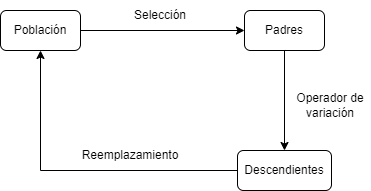
\includegraphics[scale=0.5]{figures/Algoritmos_evolutivos.png}
	\caption{Generación en algoritmos evolutivos.}
    \label{fg:alg_ev}
\end{figure}

El algoritmo \ref{alg:ev} ilustra este procedimiento.

\begin{Ualgorithm}[H]
    \label{alg:ev}
    \small
    \DontPrintSemicolon
    \KwOut{Mejor solución encontrada}
    Generar$(P_0)$ \tcp{Generación de la población inicial}
    $t \longleftarrow 0$\;
    \While{No se cumpla la condición de parada}{
        Evaluar($P_t$)
        $P_t' \longleftarrow$ Seleccionar($P_t$)\;
        $P_t' \longleftarrow$ Reproducción($P_t'$)\;
        Evaluar($P_t'$)\;
        $P_{t+1} \longleftarrow$ Reemplazar($P_t, P_t'$)\;
        $t \longleftarrow t + 1$\;
    }
\end{Ualgorithm}

\subsubsection{Algoritmos genéticos}

Los \emph{algoritmos genéticos} son algoritmos de optimización, búsqueda y aprendizaje inspirados en los procesos de evolución natural y evolución genética.

Estos algoritmos suelen aplicar como operador de variación un operador de cruce a las dos soluciones (cromosomas) que juegan un papel importante, además de un operador de mutación que modifica aleatoriamente el contenido del individuo (gen) para fomentar la diversidad. Los algoritmos genéticos usan una selección probabilística. El reemplazamiento es generacional, esto es, los padres serán reemplazados por sus descendientes. El operador de cruce se basa en un cruce uniforme o por segmento fijo, mientras que la mutación, con cierta probabilidad, determinará si algún gen puede mutar.

El operador de cruce es un operador binario y, a veces, $n$-ario. Este operador se basa en adquirir las características de los dos padres y generar un descendiente. La principal característica de este operador es la \emph{heredabilidad}, pues crea un cromosoma a partir de los genes heredados de los padres. Esto es, el descendiente tendrá una recombinación de las características de sus padres. Los padres cruzarán con una cierta probabilidad $p_c$. El operador de cruce debe producir soluciones válidas.

El operador de mutación es un operador unario que actúa sobre un solo individuo. Las mutaciones representan pequeños cambios de los individuos seleccionados. La probabilidad $p_m$ define la probabilidad de mutar cada elemento (gen) de la representación. Este operador debe garantizar que cualquier solución estará en el espacio de búsqueda y que sea válida. Con la mutación conseguimos introducir diversidad en los individuos de una población.

El algoritmo \ref{alg:gen} ilustra este procedimiento.

\begin{Ualgorithm}[H]
    \label{alg:gen}
    \small
    \DontPrintSemicolon
    \KwOut{Mejor solución encontrada}
    Generar$(P_0)$ \tcp{Generación de la población inicial}
    $t \longleftarrow 0$\;
    \While{No se cumpla la condición de parada}{
        Evaluar($P_t$)
        $P_t' \longleftarrow$ Seleccionar($P_t$)\;
        $P_t' \longleftarrow$ OperadorCruce($P_t'$)\;
        $P_t' \longleftarrow$ OperadorMutación($P_t'$)\;
        $P_{t+1} \longleftarrow$ Reemplazar($P_t, P_t'$)\;
        $t \longleftarrow t + 1$\;
    }
\end{Ualgorithm}

Este modelo es elitista y produce una convergencia rápida cuando se reemplazan los peores cromosomas de la población.
